% Figura Anexo III: los tres canales por los que un aumento del gasto público llega al consumo en el modelo NEK-2
\documentclass[tikz,border=3pt]{standalone}
\usepackage[T1]{fontenc}
\usepackage[utf8]{inputenc}
\usepackage{amsmath}
\usetikzlibrary{arrows.meta,calc,positioning}
\begin{document}
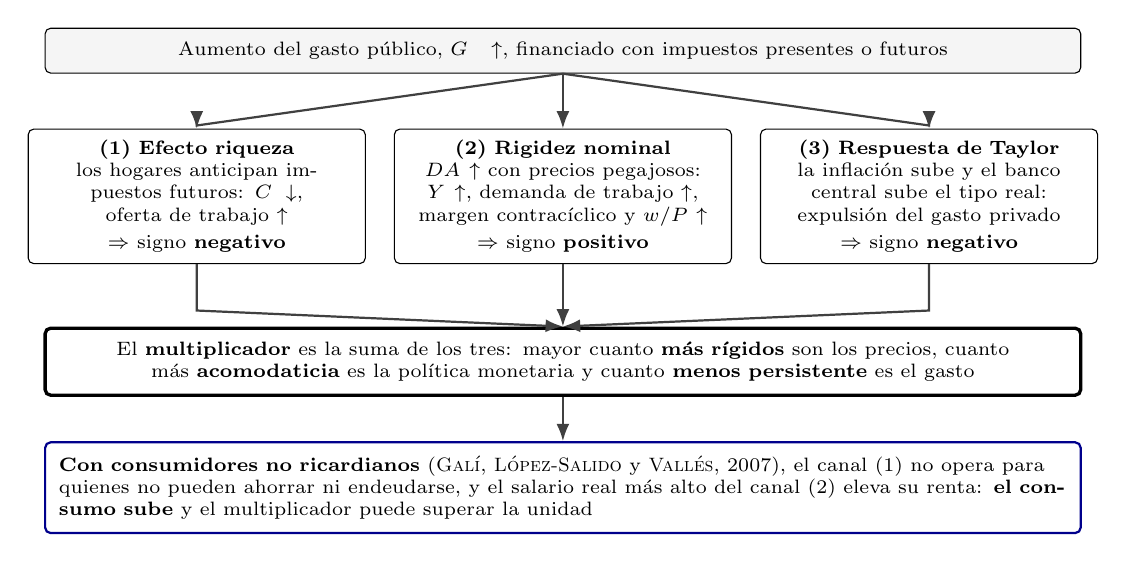
\begin{tikzpicture}[>={Latex[length=2.2mm]}, font=\footnotesize,
  caja/.style={draw, rounded corners=2pt, align=center, inner sep=4pt, text width=4.0cm, font=\scriptsize},
  ancha/.style={draw, rounded corners=2pt, align=center, inner sep=5pt, text width=12.8cm, font=\scriptsize},
  final/.style={draw, very thick, rounded corners=2pt, align=center, inner sep=5pt, text width=12.8cm, font=\scriptsize},
  lateral/.style={draw=blue!55!black, thick, rounded corners=2pt, align=left, inner sep=5pt, text width=12.8cm, font=\scriptsize},
  fl/.style={->, thick, gray!50!black}]
  \node[ancha, fill=gray!8] (g) at (0,0) {Aumento del gasto público, $G\uparrow$, financiado con impuestos presentes o futuros};
  \node[caja] (c1) at (-4.65,-1.85) {\textbf{(1) Efecto riqueza}\\los hogares anticipan impuestos futuros: $C\downarrow$, oferta de trabajo $\uparrow$\\[2pt]$\Rightarrow$ signo \textbf{negativo}};
  \node[caja] (c2) at (0,-1.85) {\textbf{(2) Rigidez nominal}\\$DA\uparrow$ con precios pegajosos: $Y\uparrow$, demanda de trabajo $\uparrow$, margen contracíclico y $w/P\uparrow$\\[2pt]$\Rightarrow$ signo \textbf{positivo}};
  \node[caja] (c3) at (4.65,-1.85) {\textbf{(3) Respuesta de \textsc{Taylor}}\\la inflación sube y el banco central sube el tipo real: expulsión del gasto privado\\[2pt]$\Rightarrow$ signo \textbf{negativo}};
  \draw[fl] (g.south) -- (-4.65,-0.95) -- (c1.north);
  \draw[fl] (g.south) -- (c2.north);
  \draw[fl] (g.south) -- (4.65,-0.95) -- (c3.north);
  \node[final] (m) at (0,-3.95) {El \textbf{multiplicador} es la suma de los tres: mayor cuanto \textbf{más rígidos} son los precios, cuanto más \textbf{acomodaticia} es la política monetaria y cuanto \textbf{menos persistente} es el gasto};
  \draw[fl] (c1.south) -- (-4.65,-3.3) -- (m.north);
  \draw[fl] (c2.south) -- (m.north);
  \draw[fl] (c3.south) -- (4.65,-3.3) -- (m.north);
  \node[lateral] (nr) at (0,-5.55) {\textbf{Con consumidores no ricardianos} (\textsc{Galí}, \textsc{López-Salido} y \textsc{Vallés}, 2007), el canal (1) no opera para quienes no pueden ahorrar ni endeudarse, y el salario real más alto del canal (2) eleva su renta: \textbf{el consumo sube} y el multiplicador puede superar la unidad};
  \draw[fl] (m.south) -- (nr.north);
\end{tikzpicture}
\end{document}
